\subsection{Derivaci\'on Heur\'istica de la Ecuaci\'on Cin\'etica}

Para la derivaci\'on de la ecuaci\'on cin\'etica o la ecuaci\'on de Boltzmann seguimos la siguiente estrategia tal y como lo plantea \cite{freidberg2014}

\begin{enumerate}
  \item Derivar la conservaci\'on de part\'iculas de un fluido simple en un espacio de fase 3-D.
  \item Generalizar a 6-D y divir las interacciones en aquellas de corto y largo alcance.
  \item A\~nadir el efecto de colisiones donde se asume \'unicamente \textbf{colisiones binarias}.
\end{enumerate} 

\subsubsection{Conservaci\'on de part\'iculas en un espacio de fase 3-D}

Primero consideraremos el caso 1-D \textbf{sin fuentes ni sumideros} en tal caso para un elemento infinitesimal de volumen 

\begin{equation*}
\text{Part\'iculas ganadas} = \text{Part\'iculas que entran - Part\'iculas que salen}
\end{equation*}

Sea $n(x_1, t)$ la densidad de part\'iculas y $\Gamma_{1} = nv_{1}$ el flujo de part\'iculas que entran al volumen.  

\begin{eqnarray}
  \text{Part\'iculas ganadas en un tiempo }  \Delta t &=& [n(x_1, t + \Delta t) - n(x_1,t)]\Delta x_1\Delta x_2\Delta x_3 \nonumber \\
  \text{Part\'iculas entran en un tiempo } \Delta t &=& (\text{flujo que entra})(\text{\'area})\Delta t = \Gamma_{1}\big{|}_{x_1 - \Delta x_1/2} \Delta x_2\Delta x_3 \nonumber\\
  \text{Part\'iculas salen en un tiempo } \Delta t &=& (\text{flujo que sale})(\text{\'area})\Delta t = \Gamma_{1}\big{|}_{x_1 + \Delta x_1/2}\Delta x_2\Delta x_3 \nonumber
\end{eqnarray}

\begin{figure}[htb!]
  \centering
  \label{fig:box}
  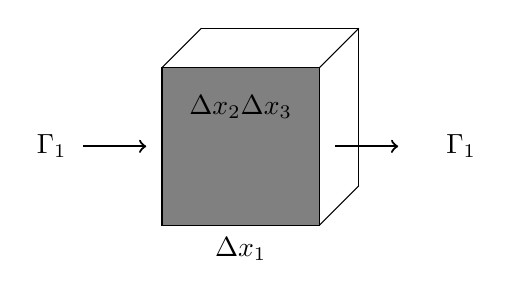
\begin{tikzpicture}
    \node at (-1.4,1) {$\Gamma_{1}$};
    \draw[->, thick] (-1,1) -- (-0.2,1);
    \draw[->, thick] (2.2, 1) -- (3,1);
    \node at (3.8,1) {$\Gamma_{1}$};
    \fill[gray] (0,0) rectangle (2,2);
    \draw (0,0) rectangle (2,2);
    \draw (2, 0) -- (2.5,0.5);
    \draw (2.5,0.5) -- (2.5, 2.5);
    \draw (0.5,2.5) -- (2.5,2.5);
    \draw (0,2) -- (0.5,2.5);
    \draw (2,2) -- (2.5,2.5);
    \node at (1,-0.3) {$\Delta x_1$};
    \node at (1, 1.5) {$\Delta x_2 \Delta x_3$};
  \end{tikzpicture}
  \caption{Elemento de volumen en un espacio de fase 3-D con un flujo en la direcci\'on $x_1$.}
\end{figure}

Expandiendo las expresiones en series de Taylor a primer orden

\begin{eqnarray}
  \text{Ganadas }\Delta t &=& [ n(x_1,t) + \partial_t n(x_1,t) - n(x_1, t)]\Delta x_1\Delta x_2\Delta x_3 \nonumber\\ 
                          &=& \left\{ \left[\Gamma_{1}\big{|}_{x_1} - \frac{\Delta x_1}{2}(\partial_{1}\Gamma_{1})\big{|}_{x_1}\right] - \left[\Gamma_{1}\big{|}_{x_1} + \frac{\Delta x_1}{2}(\partial_{1}\Gamma_{1})\big{|}_{x_1}\right]\right\}\Delta x_2\Delta x_3\nonumber
  \end{eqnarray}

De all\'i se obtiene la expresi\'on

\begin{equation*}
  \partial_{t} n = -\partial_{1}\Gamma_{1}
\end{equation*}

La generalizaci\'on al caso 3-D es inmediata, tal que 

\begin{equation*}
  \partial_t n(\textbf{x}, t) + \nabla_\textbf{x}\cdot\pmb{\Gamma}(\textbf{x},t) = 0
\end{equation*}

\subsubsection{Generalizaci\'on a un espacio de fase 6-D}

En un espacio de fase 6-D conformado por los puntos (\textbf{x}, \textbf{v}) se procede a generalizar de forma que 

\begin{eqnarray*}
  n(\textbf{x},t) \rightarrow f(\textbf{x}, \textbf{v},t) \text{ (6-D) } \quad \quad \quad \quad \text{densidad del espacio de fase}\\
  \Delta x_1\Delta x_2\Delta x_3 \rightarrow \Delta x_{1}\Delta x_2\Delta x_3\Delta v_{1}\Delta v_{2}\Delta v_{3} \text{ (6-D) } \text{elemento de volumen}
\end{eqnarray*}

N\'otese la independencia entre $\textbf{x}$ y $\textbf{v}$, por lo que en general $\textbf{a} = \textbf{a}(\textbf{x},\textbf{v}, t)$. Ahora generalizamos tomando en cuenta fuentes y sumideros para cada elemento del volumen del espacio de fase. Primero se considerara el caso donde solo haya moviento en el espacio de fase en las direcciones $x_1$ y $v_{1}$, luego, de manera an\'aloga al caso en el espacio 3-D ser\'a f\'acil generalizar las expresiones. Imaginemos al espacio f\'isico y al espacio de velocidades la geometr\'ia del problema est\'a dada por 

\begin{figure}[h!]
  \label{fig:fasespace}
  \centering
  \begin{subfigure}{0.49\textwidth}
    \begin{tikzpicture}
      \draw (0,0) rectangle (3,2);
      \node at (-1.4,1) {$v_{1}$};
      \draw[->, thick] (-1, 1) -- (-0, 1);
      \draw[->, thick] (3,1) -- (4,1);
      \node at (4.4,1) {$v_{1}$};
      \node at (0,-0.5) {$x_1 - \Delta x_1/2 $};
      \node at (3,-0.5) {$x_1 + \Delta x_1/2 $};
    \end{tikzpicture}
    \caption{}
  \end{subfigure}
  \begin{subfigure}{0.49\textwidth}
    \begin{tikzpicture}
      \draw (0,0) rectangle (3,2);
      \node at (-1.4,1) {$a_{1}$};
      \draw[->, thick] (-1, 1) -- (-0, 1);
      \draw[->, thick] (3,1) -- (4,1);
      \node at (4.4,1) {$a_{1}$};
      \node at (0,-0.5) {$v_{1} - \Delta v_{1}/2 $};
      \node at (3,-0.5) {$v_{1} + \Delta v_{1}/2 $};
    \end{tikzpicture}
    \caption{}
  \end{subfigure}
  \caption{(a) flujo de part\'icula en el espacio f\'isico. (b) flujo de part\'iculas en el espacio de velocidades.}
\end{figure}

\begin{equation*}
  \text{part\'iculas ganadas} = \text{entran} - \text{salen} + \text{fuentes} - \text{sumideros}
\end{equation*}

De está definimos

\begin{eqnarray}
  \text{ganadas en } \Delta t &=& [f(x_1, v_{1}, t + \Delta t) - f(x_1, v_{1}, t)]\Delta\textbf{x}\Delta\textbf{v}\nonumber\\
  \text{entran en espacio f\'isico} &=& \Delta x_{2}\Delta x_{3}\Delta t[v_{1}fd\textbf{v}]_{x_1 - \Delta x_1/2} \nonumber\\
  \text{salen en espacio f\'isico} &=& \Delta x_{2}\Delta x_{3}\Delta t[v_{1}fd\textbf{v}]_{x_1 + \Delta x_1/2} \nonumber\\
  \text{aceleran en espacio de velocidad} &=& \Delta v_{2}\Delta v_{3}\Delta t[a_{1}fd\textbf{x}]_{v_{1} - \Delta v_{1}/2} \nonumber\\
  \text{aceleran fuera del espacio de velocidad} &=& \Delta v_{2}\Delta v_{3}\Delta t[a_{1}fd\textbf{x}]_{v_{1} + \Delta v_{1}/2} \nonumber\\
  \text{fuentes} - \text{sumideros} &=& s\Delta \textbf{x} \Delta\textbf{v}\Delta t \nonumber
\end{eqnarray}

Al aplicar las correspondientes expansiones de Taylor al rededor de $t$, $x_1$ y $v_1$ se obtiene 

\begin{equation*}
  \partial_t f = -\partial_{1}(v_1 f) - \partial_{v_1} (a_1 f) + s
\end{equation*}

Adem\'as recordando que $\partial_{i}v_j = 0$ se obtiene

\begin{equation*}
  \partial_t f + v_1\partial_{1}f + a_1\partial_{v_1} f + f\partial_{v_1}a_1 = s
\end{equation*}
  
La generalizaci\'on al espacio 6-D es simple, tal que 

\begin{equation*}
  \partial_t f(\textbf{x},\textbf{v}, t) + \textbf{v}\cdot\nabla f(\textbf{x}, \textbf{v}, t) + \textbf{a}\cdot\nabla_{\textbf{v}} f(\textbf{x}, \textbf{v}, t)= -f(\textbf{x}, \textbf{v}, t)\nabla_\textbf{v}\cdot \textbf{a} + s 
\end{equation*}

\subsubsection{Ecuaci\'on Cin\'etica de Boltzmann}

Considerando el caso de inter\'es, el plasma, el t\'ermino $\textbf{a}$ puede ser dividido en dos partes, aceleraci\'on por interacciones de corto alcance $\textbf{a}_c$ y por interacciones de largo alcance $\textbf{a}_l$ tal que 

\begin{equation*}
  \textbf{a} = \textbf{a}_s + \textbf{a}_l
\end{equation*}

El cr\'iterio para definir el alcance de las interacciones es el radio de Debye $\lambda_D$. Se c\'ataloga como una fuerza de corto alcance a aquellas que se dan en un radio mucho menor al de Debye $r \ll \lambda_D$ y en este caso se asumen solo colisiones de Coulomb las cuales debido al apantallamiento de Debye son despreciales fuera de la esfera de Debye $V_D$. 

Se hace una primera aproximaci\'on en la que se limitan las colisiones a ocurrir en un punto tan pequeño que la posici\'on de la part\'icula no cambia en el espacio f\'isico ni antes ni despu\'es de una colisi\'on. Adem\'as, la velocidad de la part\'icula cambia finitamente. Es decir, el resultado de una colisi\'on no puede hacer que la velocidad se dispare al infinito. Entonces consideramos, una colisi\'on en un espacio de fase 6-D implica que $\textbf{x}$ no cambia y $\textbf{v}$ puede salir del elemento de volumen en el espacio de velocidades, es decir, el momento de la part\'icula cambia. 

Por otro lado, se desprecian los efectos de las colisiones no binarias, es decir, las colisiones entre tres o m\'as part\'iculas. Tambi\'en, se asume que el n\'umero de part\'iculas en un $V_D$ este dentro del l\'imite estad\'istico y las escalas dimensionales y temporales del problema son tales que, $V_D \ll L$ y $\tau \ll \tau_{pe}$ donde $\tau_{pe}$ es el periodo electr\'onico del plasma. 

Consideremos primero las interacciones de largo alcance

\begin{equation*}
  \textbf{a}_{l,\alpha} = \frac{Ze}{m_\alpha}(\textbf{E} + \textbf{v}\times\textbf{B})
\end{equation*}

Para estas interacciones de largo alcance se toma solo el promedio tal que los campos sean suaves y no var\'ien abruptamente, por lo que $\textbf{E}$ y $\textbf{B}$ solo dependen de $\textbf{x}$. De all\'i que

\begin{eqnarray}
  \nabla_\textbf{v}\cdot\textbf{a}_{l, \alpha} &=& \frac{Ze}{m_\alpha}\nabla_\textbf{v}\cdot(\textbf{E}(\textbf{x},t) + \textbf{v}\times\textbf{B}(\textbf{x},t))\nonumber\\
                                   &=& \frac{Ze}{m_\alpha}\left[\nabla_\textbf{v}\cdot \textbf{E} + \nabla_\textbf{v}\cdot(\textbf{v}\times\textbf{B})\right] \nonumber\\
                                   &=& \frac{Ze}{m_\alpha}[\partial_{v_\mu} (\epsilon_{\mu\nu\rho} v_{\nu}B_{\rho})] \nonumber \\
                                   &=& \frac{Ze}{m_\alpha}\epsilon_{\mu\nu\rho}(B_\rho \partial_{v_\mu}v_{\nu} + v_\nu\cancel{\partial_{v_\mu}B_\rho}) \nonumber \\
                                   &=& \frac{Ze}{m_\alpha}\epsilon_{\mu\nu\rho}(B_\rho\delta_{\mu\nu})\nonumber \\
                                   &=& \frac{Ze}{m_\alpha}\cancel{\epsilon_{\mu\mu\rho}}B_\rho = 0
\end{eqnarray}

Bajo los supuestos anteriores, y agregando las interacciones de corto alcance como las \'unicas fuentes y/o sumideros para part\'iculas de la especie $\alpha$, la funci\'on de distribuci\'on cumple 

\begin{equation}
  \partial_t f_\alpha + \textbf{v}\cdot\nabla f_\alpha + \frac{Ze}{m_\alpha}(\textbf{E} + \textbf{v}\times\textbf{B})\cdot\nabla f_\alpha = C_\alpha
\end{equation}

Aqu\'i se reemplazo el t\'ermino de fuentes y sumideros por $s = C_\alpha$ que toma en cuenta \'unicamente colisiones binarias tal que, siendo $C_\alpha$ la suma del operador de colisiones binarias $C_{\alpha\beta}$ sobre todas las part\'iculas $\alpha$

\begin{equation}
  s \rightarrow C_\alpha = (\delta_t f_\alpha)_c = \sum_\alpha C_{\alpha\beta}(\textbf{x}, \textbf{v},t)
\end{equation}

donde $C_{\alpha\beta}$ representa el cambio en $f_\alpha$ debido a colisiones con las especies $\beta$. Es importante notar que todas las interacciones entre part\'iculas a nivel microsc\'opico son tomadas en cuenta dentro del operador de colisiones.
